\begin{figure*}[htbp]
    \centering
    \begin{subfigure}[b]{0.32\textwidth}
       \centering
       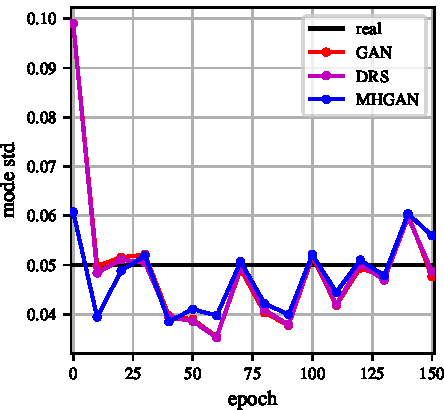
\includegraphics[width=1.75in]{figures/std.pdf}
       \caption{mode std.~dev.}
       \label{fig:std}
    \end{subfigure}
    \begin{subfigure}[b]{0.32\textwidth}
       \centering
       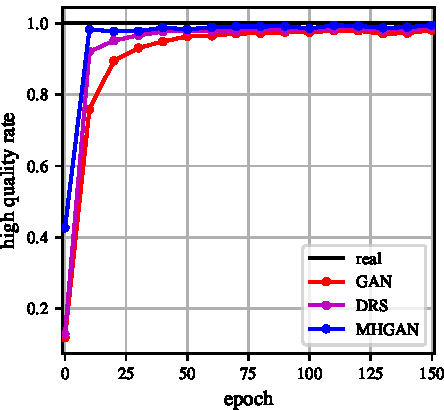
\includegraphics[width=1.75in]{figures/hqr.pdf}
       \caption{high quality rate}
       \label{fig:hqr}
    \end{subfigure}
    \begin{subfigure}[b]{0.32\textwidth}
       \centering
       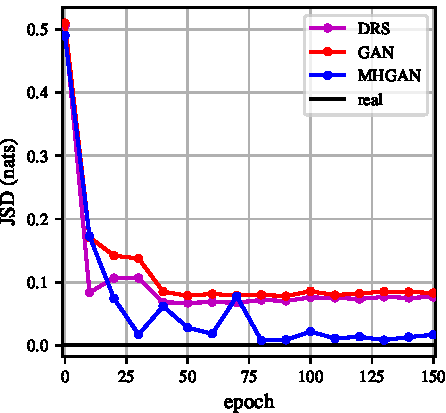
\includegraphics[width=1.75in]{figures/jsd.pdf}
       \caption{Jensen-Shannon divergence}
       \label{fig:jsd}
    \end{subfigure}
    \caption{{\small
    Results of the MH-GAN experiments on the mixture of 25 Gaussians example.
    On the left, we show the standard deviation of samples within a single mode.
    The black lines represent values for the true distribution.
    In the center, we show the high quality rate (samples near a real mode) across different GAN setups.
    On the right, we show the Jensen-Shannon divergence (JSD) between the distribution on the nearest mode vs a uniform, which is the generating distribution on mixture components.
    The MH-GAN shows, on average, a $5 \times$ improvement in JSD over DRS\@.
    We considered adding error bars to these plots via a bootstrap analysis, but the error bars are too small to be visible.
    }}
    \label{fig:mog_metrics}
\end{figure*}
